\chapter{Formal Analysis using Alloy}

Here we present a possible formal model for the TrackMe system. The model is built using the Alloy specifications.

We modeled mainly the Data4Help and Track4Run services, with just a small part dedicated to AutomatedSOS. In the intent not to overwhelm the model with numerous signatures and attributes, some features of the system have been left out and we focused on the request mechanisms, the run organization and the anonymity of data in group requests.
In particular, we modeled an anonymous identifier that permits the identification of a user in a group, without accessing his personal information.

\vspace{12mm}

\begin{minted}[breaklines, breaklines]{alloy}

open util/integer
open util/boolean
open util/time

sig Username{}
sig CF {}
sig VAT {}

abstract sig RegisteredUser {
	username: one Username,
}

sig User extends RegisteredUser {
	cf: one CF,
	data: some Record,
	automated_sos: one Bool
}

sig ThirdParty extends RegisteredUser {
	vat: one VAT,
	// For simplicity we consider only positive requests
	positive_requests: set Request
}

sig HealthStatus {
	heartBeat: lone Int,
	bloodPressure: lone Int,
	bodyTemperature: lone Int, 
	stepCounter: lone Int
}

sig Position {
	latitude: one Int,
	longitude: one Int
}

sig Record {
	timestamp: one Time,
	location: one Position,
	health: one HealthStatus,
	anon_id: one Int
}

sig Description {}
sig EmergencyRecord extends Record {
	user: one User,
	description: one Description
} {
	this in user.data
}

abstract sig Status {}
// only one of these can be true
one sig Accepted extends Status{}
one sig Pending extends Status{}
one sig Refused extends Status{}

abstract sig Request {
	sender: one ThirdParty,
}

sig UserRequest extends Request {
	receiver: one User,
	status: one Status,
	obtained_data: lone Record
} {
	// Data is present only if the request is accepted by the user
	(status = Pending or status = Refused) implies no obtained_data
}

sig GroupRequest extends Request{
	restrictions: Restrictions,
	allowed: one Bool,
	obtained_data: set Record
} {
	// Data are present only if the request is allowed by the system
	allowed.isFalse implies no obtained_data
	allowed.isTrue implies some obtained_data
}

sig SubscriptionUserRequest extends UserRequest {}
sig SubscriptionGroupRequest extends GroupRequest {}

// Restrictions applied to group requests
sig Restrictions {
	location: lone Position,
	radius: lone Int,
	age_max: lone Int,
	age_min: lone Int
}

sig Run {
	organizer: one User,
	path: one Path,

	start_time: one Time,
	end_time: one Time,

	max_participants: one Int,
	enrolled_users: set User,
	num_spectators: one Int,

	started: one Bool,
	ended: one Bool
}

sig Path {
	starting_point: one Position,
	intermediate_points: set Position,
	ending_point: one Position
}
\end{minted}

\newpage

\begin{minted}[breaklines, breaklines]{alloy}
// CONSTRAINTS


// DATA4HELP

// Registration data for the system are unique
fact registrationDataUniqueness {
	// Unique username
	no disjoint u1, u2: RegisteredUser | u1.username = u2.username
	// Unique fiscal code
	no disjoint u1,u2: User | u1.cf = u2.cf
	// Unique VAT
	no disjoint t1,t2: ThirdParty | t1.vat = t2.vat
}

// Request status can have only one of these values: Accepted, Pending or Refused
fact requestConsistency {
	all s: Status | (s = Accepted && s != Pending && s != Refused) || (s != Accepted && s = Pending && s != Refused) || (s != Accepted && s != Pending && s = Refused) 
}

// If a request has no sender, it also has no receiver
fact noSenderNoReceiver {
	all r: Request | no r.sender implies no r.receiver
}

fact thirdPartyRequests{
	// Accepted/allowed requests are related to the third party that sent them
	all t: ThirdParty, r: Request | r in t.positive_requests implies r.sender = t

	// All the request related to a third party have been accepted/allowed
	all t: ThirdParty, r: UserRequest | r in t.positive_requests implies r.status = Accepted
	all t: ThirdParty, r: GroupRequest | r in t.positive_requests implies r.allowed.isTrue
}

// If accepted by the user, a user request contains one record of the user who accepted it
fact obtainedDataAfterAcceptance {
	all r: UserRequest | (r.status = Accepted implies one r.obtained_data) and r.obtained_data in r.receiver.data
}

// No unlinked instances
fact noUnlinked {
	all h: HealthStatus | some r: Record | h = r.health 
	all p: Position | some r: Restrictions, rec: Record | p = r.location or p = rec.location
	all r: Restrictions | some g: GroupRequest | r = g.restrictions
	all p: Path | some r: Run | p = r.path
	all d: Description | some e: EmergencyRecord | d = e.description
}

// If a record is not already associated to a user, it can not be available for requests
fact noUserNoRequest{
	all r: Record, ureq: UserRequest, greq: GroupRequest | (r not in User.data) implies (r not in ureq.obtained_data and r not in greq.obtained_data) 
}

fact uniqueAnonID {
	// Records associated with different users have different anonymous ID
	all u1, u2: User, r1, r2: Record | ((r1 in u1.data) and (r2 in u2.data) and u1 != u2) implies r1.anon_id != r2.anon_id
	// Records associated with the same user have the same anonymous ID
	all u: User, r1, r2: Record | ((r1 in u.data) and (r2 in u.data)) implies r1.anon_id = r2.anon_id
}

// Records associated with the same user have different timestamps
fact uniqueTimestampUser {
	all u: User, r1, r2: Record | ((r1 in u.data) and (r2 in u.data) and (r1 != r2)) implies r1.timestamp != r2.timestamp
}

// Considering meaningful integer values
fact possibleValues{
	all h: HealthStatus | h.heartBeat > 0 and h.bloodPressure > 0 and h.bodyTemperature > 0 and h.stepCounter >= 0
	all p: Position | p.latitude >= -90 and p.latitude <= 90 and p.longitude >= -180 and p.longitude <= 180 
	all rec: Record | rec.anon_id >= 0
	all res: Restrictions | res.radius > 0 and res.radius < 100 //km
		and res.age_max >= 18 and res.age_max < 110 and res.age_min >= 18 and res.age_min < 110
	all r: Run | r.max_participants > 0 and r.max_participants < 100 and  #r.enrolled_users > 0 and #r.enrolled_users < 100 and  r.num_spectators > 0 and r.num_spectators < 100
}


// TRACK4RUN

// The end of a run must happen after its start
fact TimeConstraints{
	all r: Run | gt[r.end_time, r.start_time]
}

// Organizer and enrolled user must be different
fact OrganizerNotEnrolled {
	all r: Run | r.organizer not in r.enrolled_users
}

// The number of users enrolled for the same run must not exceed the maximum number
// of participants set by the organizator
fact MaxParticipants {
	all r: Run | (#r.enrolled_users >= 0 and #r.enrolled_users <= r.max_participants)
}

// A run can not be finished if it is not started yet
fact noFinishedIfNotSarted {
	all r: Run | (r.ended.isTrue implies r.started.isTrue) and (r.started.isFalse implies r.ended.isFalse)
}

// A run has no spectators if it hasn't started yet or if it has already ended.
fact numSpectators {
	all r: Run | (r.started.isFalse or r.ended.isTrue) implies r.num_spectators = 0
}

// In order for a run to start, there must be at least one user enrolled
fact minPartecipants {
	all r: Run | (r.started.isTrue implies #r.enrolled_users >= 1)
}

// Intermediate points are different from the starting and ending points
fact points {
	all pa: Path | (pa.starting_point not in pa.intermediate_points and pa.ending_point not in pa.intermediate_points)
}


// AUTOMATED SOS

// An emergency record must contain at least one critical parameter
fact emergencyIfNeeded {
	all e: EmergencyRecord | e.health.heartBeat < 45 or e.health.heartBeat > 100 //bpm
		or e.health.bloodPressure < 50 or e.health.bloodPressure > 160 //mmHg
		or e.health.bodyTemperature < 33 or e.health.bodyTemperature > 40 //Celsius
}

// A health status can not be related with both a record and an emergency record
fact healthStatusConsistency {
	all e: EmergencyRecord, r: Record - EmergencyRecord | e.health != r.health
}

// Users with disabled AutomatedSOS setting do not have associated emergency records
fact noEmergencyIfSOSDisabled {
	all u: User | u.automated_sos.isFalse implies u.data - EmergencyRecord = u.data
}

\end{minted}

\newpage

\begin{minted}[breaklines, breaklines]{alloy}
// PREDICATES

pred addRecord[r, r': Record, u, u': User] {
	// preconditions
	r' not in User.data
	// postconditions
	#u.data > 0 implies (r in u.data and r'.anon_id = r.anon_id)
	u'.data = u.data + r
}

pred acceptRequest[r, r': UserRequest] {
	// preconditions
	r.status = Pending
	r in SubscriptionUserRequest implies r' in SubscriptionUserRequest
	r in UserRequest - SubscriptionUserRequest implies r' in UserRequest - SubscriptionUserRequest
	// postconditions
	r'.status = Accepted
	r' in r'.sender.positive_requests
}

pred refuseRequest[r, r': UserRequest] {
	// preconditions
	r.status = Pending
	r in SubscriptionUserRequest implies r' in SubscriptionUserRequest
	r in UserRequest - SubscriptionUserRequest implies r' in UserRequest - SubscriptionUserRequest
	// postconditions
	r'.status = Refused
	r' not in r'.sender.positive_requests
}

pred enrollToRun[r, r': Run, u: User]{
	// preconditions
	r.started = False
	#r.enrolled_users < r.max_participants // entries available
	not u in r.enrolled_users
	// postconditions
	r'.started = r.started and r'.ended = r.ended
	r'.enrolled_users = r.enrolled_users + u
	u in r'.enrolled_users
	#r'.enrolled_users <= r.max_participants
	all u': User| u' in r.enrolled_users implies u' in r'.enrolled_users
}

pred viewLiveRun[r, r': Run]{
	// precondition
	r.started.isTrue and r.ended.isFalse
	// postcondition 					
	r'.started = r.started and r'.ended = r.ended
	r'.num_spectators = r.num_spectators + 1
}

pred createRun[r: Run, o: User, p: Path, st, et: Time, max: Int]{
	// postconditions
	r.organizer = o
	r.path = p
	r.start_time = st
	r.end_time = et
	r.max_participants = max
	no r': Run | (r' != r and r'.start_time = r.start_time and r'.end_time = r.end_time and r'.path = r.path and r'.max_participants = r.max_participants)
	r.started = False
	r.ended = False
	no u: User | u in r.enrolled_users
}

pred show{
	#User = 3
	#ThirdParty = 2
	#UserRequest = 2
	#GroupRequest = 2
	#Record >= 4 and #Record <= 5
	some u: User | #u.data=2
	#HealthStatus = 5
	some r, r': Record |  r.health != r'.health
	#EmergencyRecord = 1
	#Run = 3
	#Position > 4
	#Path = 3
	
	some r: Record | r not in User.data
	some ureq: UserRequest | ureq.status = Accepted
}


run show for 10 but 9 Int

run addRecord for 6

run acceptRequest for 3

run refuseRequest for 3

run enrollToRun for 3

run viewLiveRun for 3

run createRun for 4

\end{minted}

\newpage

\begin{figure}[H]
    \centering
    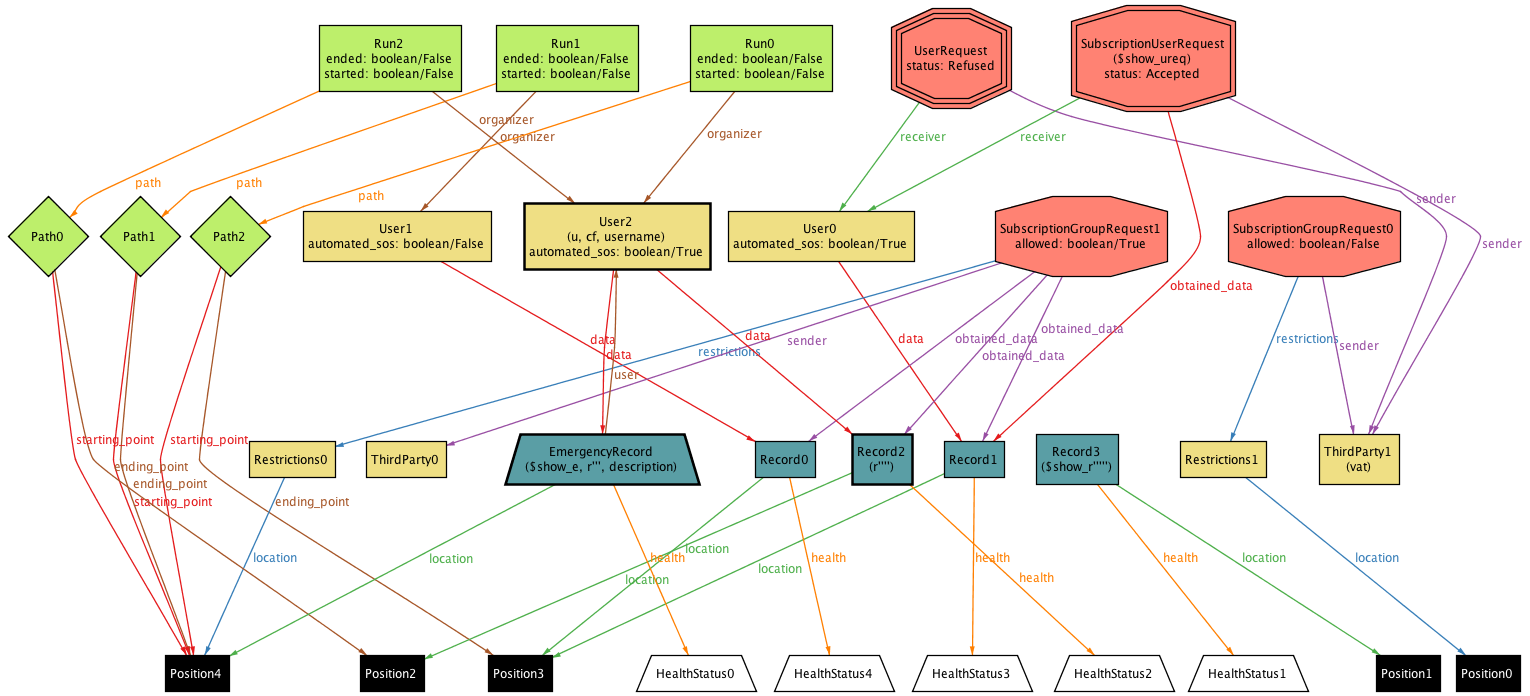
\includegraphics[angle=90, scale=0.4]{./Pictures/alloy/alloy-world.png}
\end{figure}


